\section{Methods and Implementation}\label{methods and implementation}

This section presents different processing techniques with the aim of solving the task at hand. Images will show the result, and the improvement is discussed. 

{\color{red}Explanation of kernel size, structuring element..????}


\subsection{Median Filter}
The median filter is a nonlinear digital filtering technique used to remove noise while preserving edges in images. The median filter algorithm runs through each pixel in the image and replaces the value with the median of neighboring pixel values. The neighboring pixels is located in a square neighborhood around the evaluated pixel. Each channel of a multi-channel image is processed independently. 

\begin{figure}[h]
    \centering
    \begin{subfigure}{0.5\textwidth}
        \centering
        \includegraphics[width=.9\linewidth]{Images/original_fish_image}
        \caption{Original Image}
    \end{subfigure}%
    \begin{subfigure}{.5\textwidth}
        \centering
        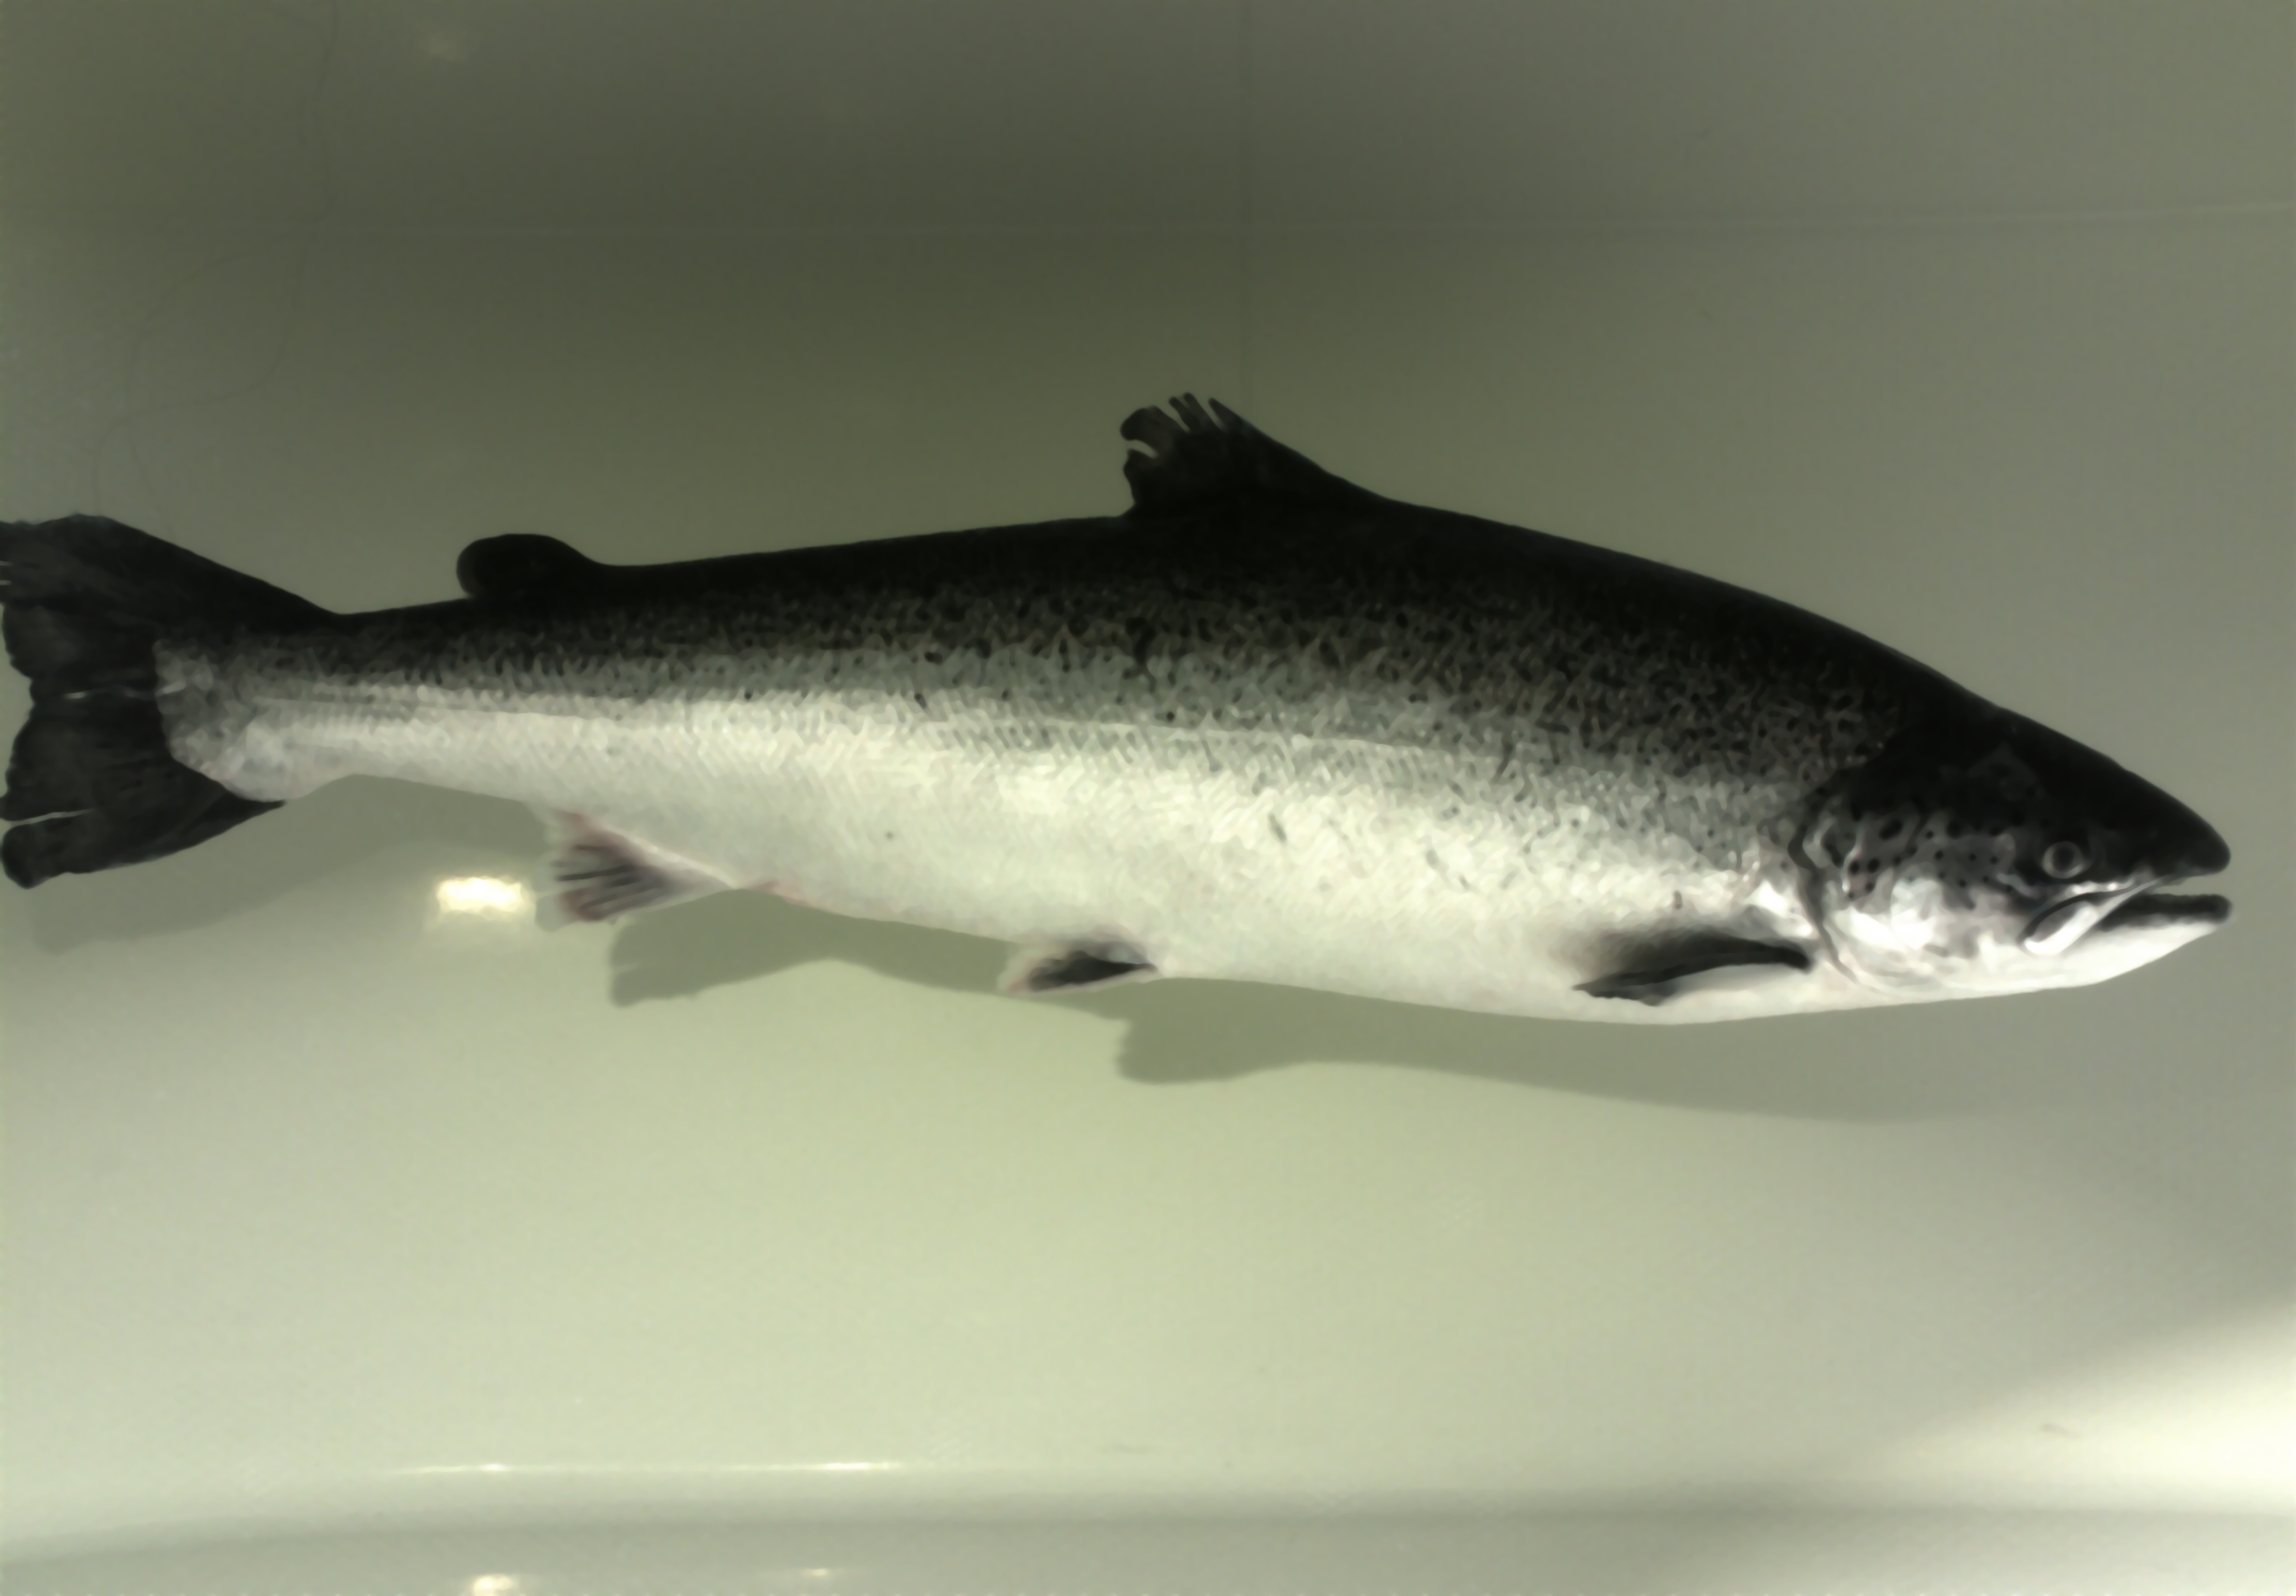
\includegraphics[width=.9\linewidth]{Images/median_filter}
        \caption{Median Filter}
    \end{subfigure}
    \caption{Example of median filtering}
    \label{fig:median_filter}
\end{figure}

It is seen from the images in figure \ref{fig:median_filter} that both the background and the black dots on the fish are smoothed out but the edges are preserved. Small particles is also removed; for example it is possible to see that the white particle under the fish is gone. The median filter used on this image has kernel size 9, and it was filtered four times in a row. When filtering several times in a row instead of increasing the kernel size the image will not get as blurry and small particles will still be removed.


\subsection{Bilateral Filter}
The bilateral filter is, just as the median filter, a nonlinear digital filter used to remove noise, while preserving sharp edges. Each pixel in an image is replaced by a weighted average of intensity values from neighboring pixels. The weight does not only depend on distance, but also on the radiometric differences such as color intensity or depth distance. 

{\color{red}Add bilateral image instead of median filter image}

\begin{figure}[h]
    \centering
    \begin{subfigure}{0.5\textwidth}
        \centering
        \includegraphics[width=.9\linewidth]{Images/original_fish_image}
        \caption{Original Image}
    \end{subfigure}%
    \begin{subfigure}{.5\textwidth}
        \centering
        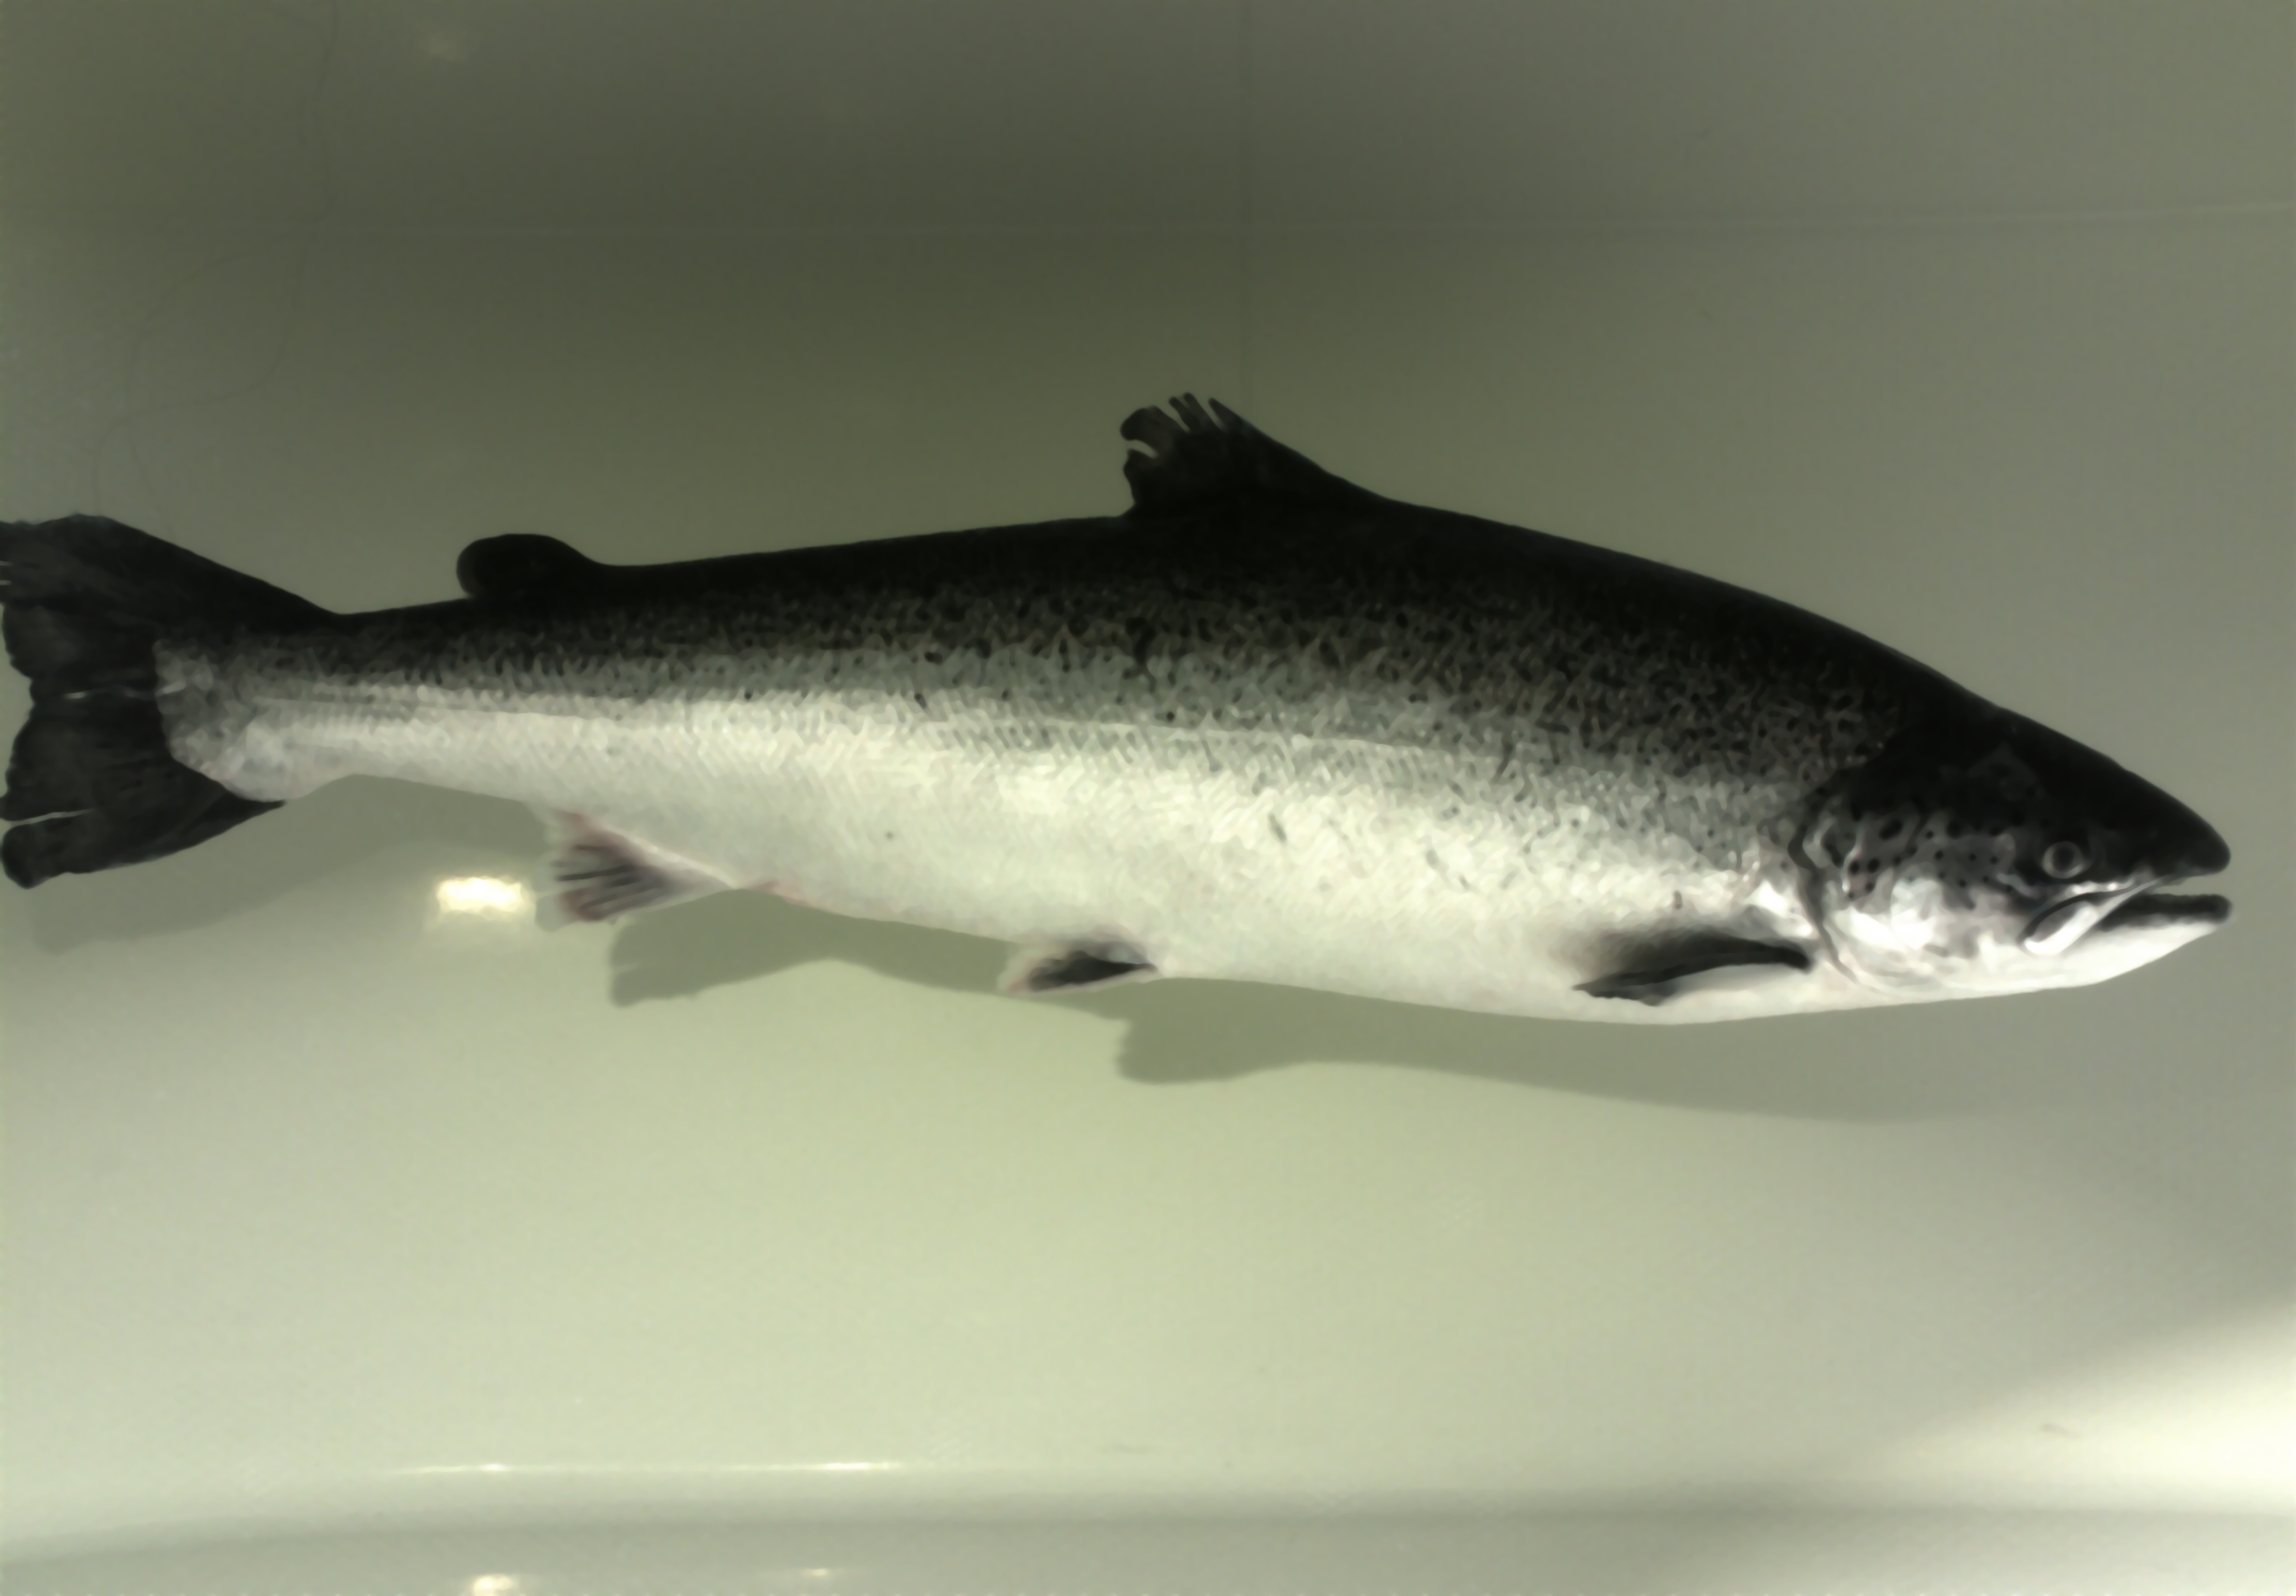
\includegraphics[width=.9\linewidth]{Images/median_filter}
        \caption{Bilateral Filter}
    \end{subfigure}
    \caption{Example of bilateral filtering}
    \label{fig:bilateral_filter}
\end{figure}

From figure \ref{fig:bilateral_filter} it is possible to see that the edges are well preserved while small particles are removed from the image. The image was filtered with kernel size {\color{red}????}, and it was filtered {\color{red}?????} times in a row.


\subsection{Eroding and Dilating}
Erosion and dilation are two morphological operators. Eroding an image will enhance the black objects in an image, while dilating will enhance the white objects in an image. It uses a structuring element which decides how and how much the objects should change. 


\subsection{Shadow Removal}
Simple shadow removal can be done by transforming the color space of the image from RBG to HSV and then setting the value component of each pixel to a constant value. What this really does is even out all grey tones in the image, as is shown in figure \ref{fig:shadow_removal}.

\begin{figure}[h]
    \centering
    \begin{subfigure}{0.5\textwidth}
        \centering
        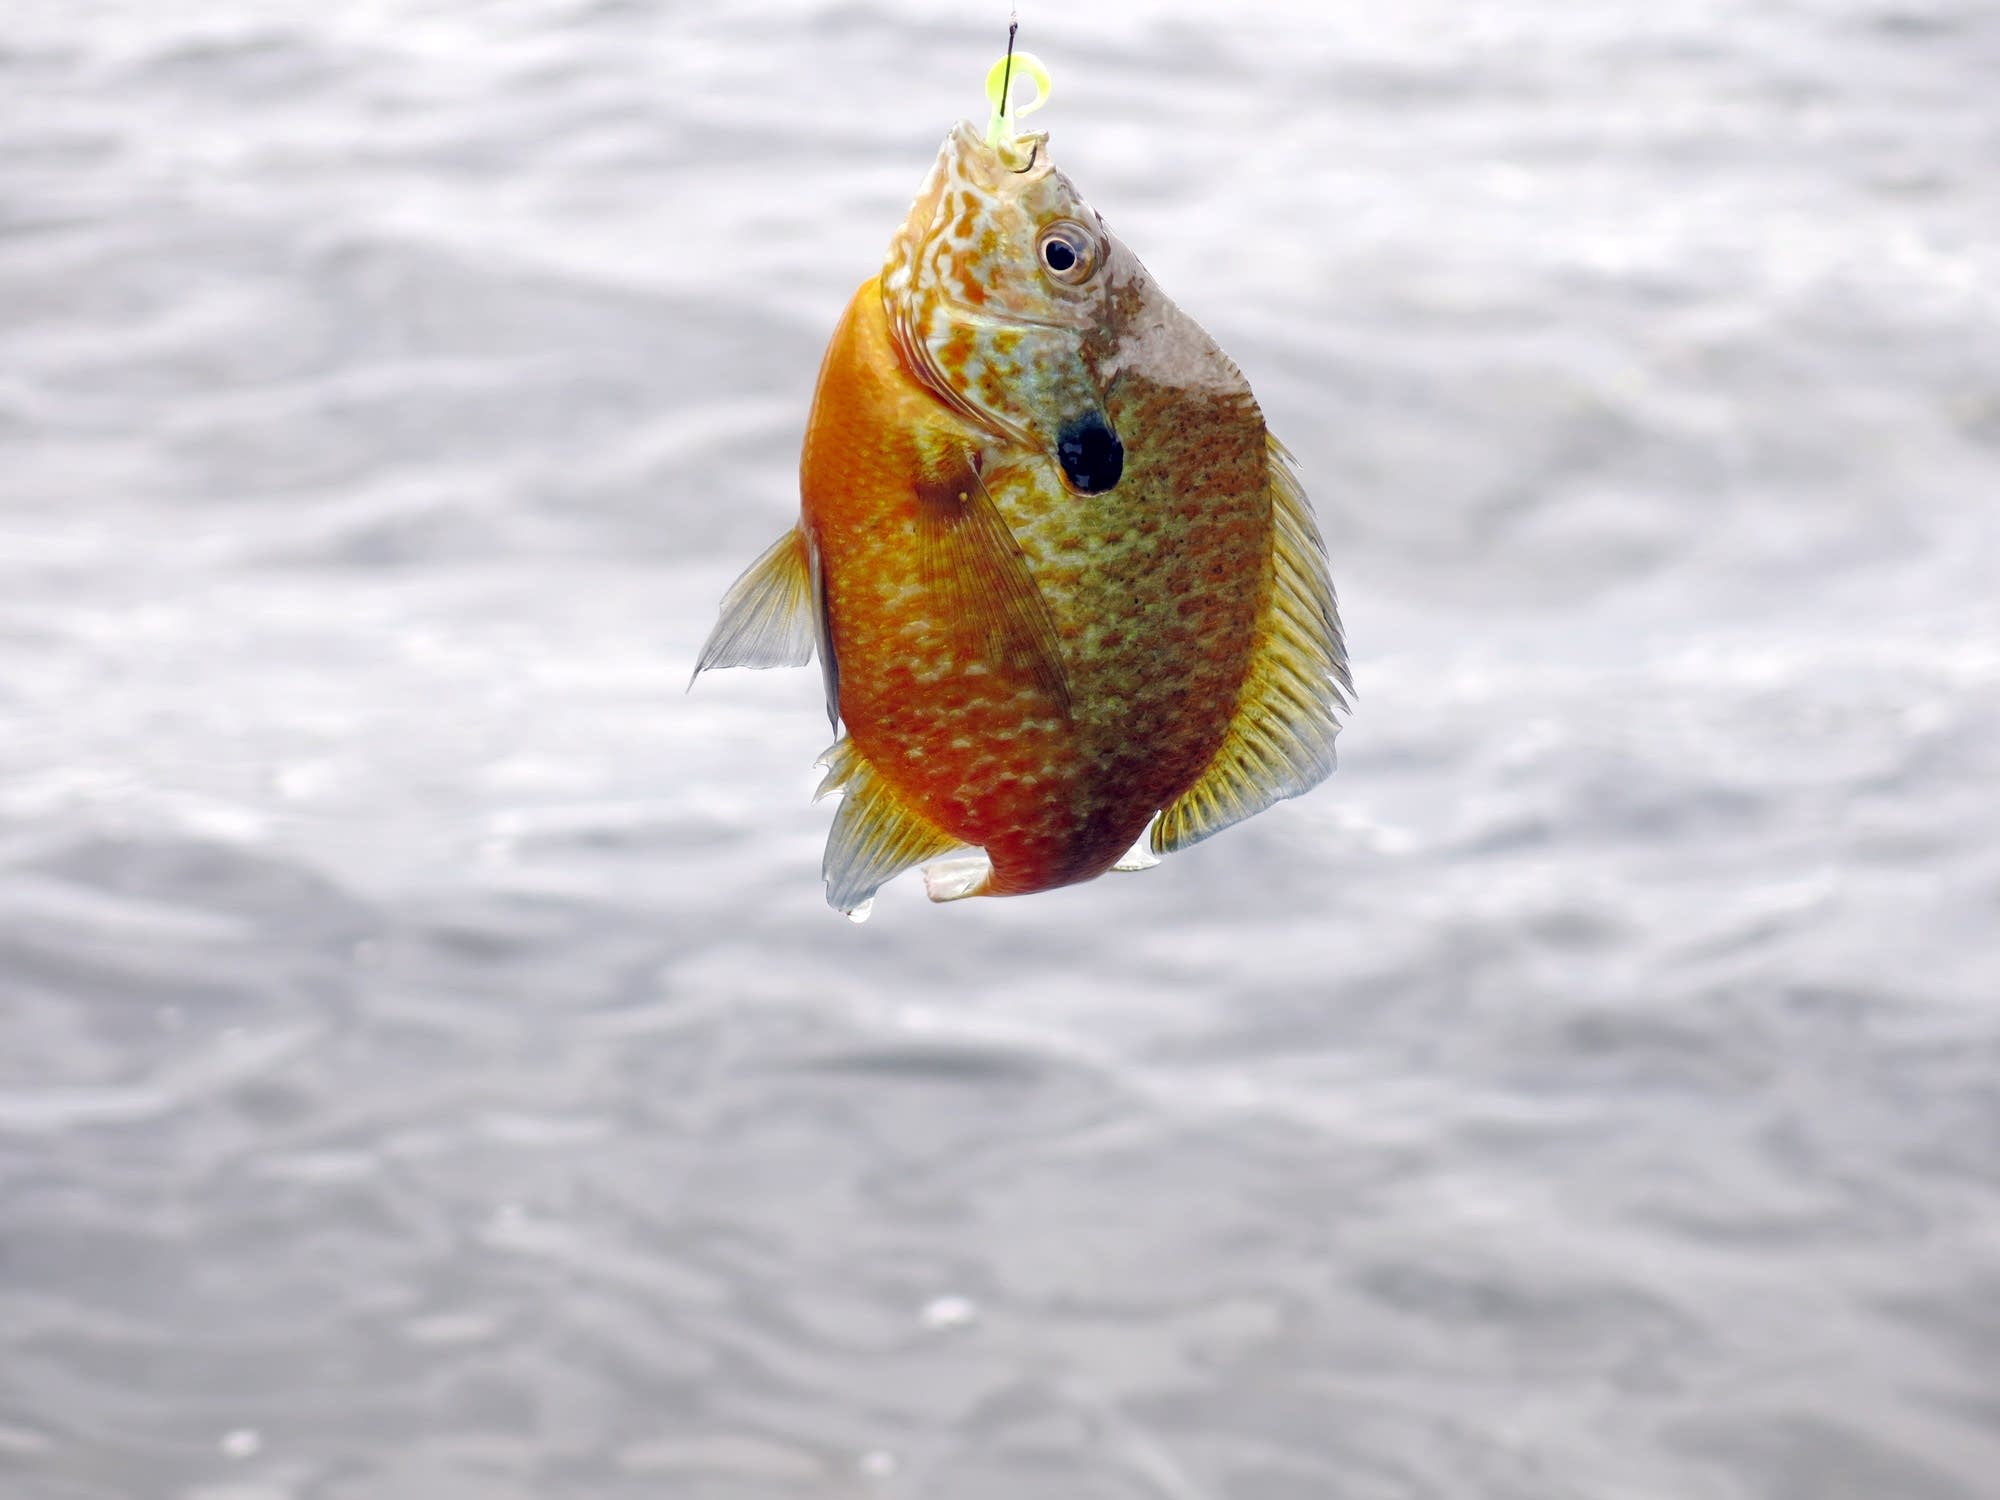
\includegraphics[width=.9\linewidth]{Images/colorfish}
        \caption{Original Image}
    \end{subfigure}%
    \begin{subfigure}{.5\textwidth}
        \centering
        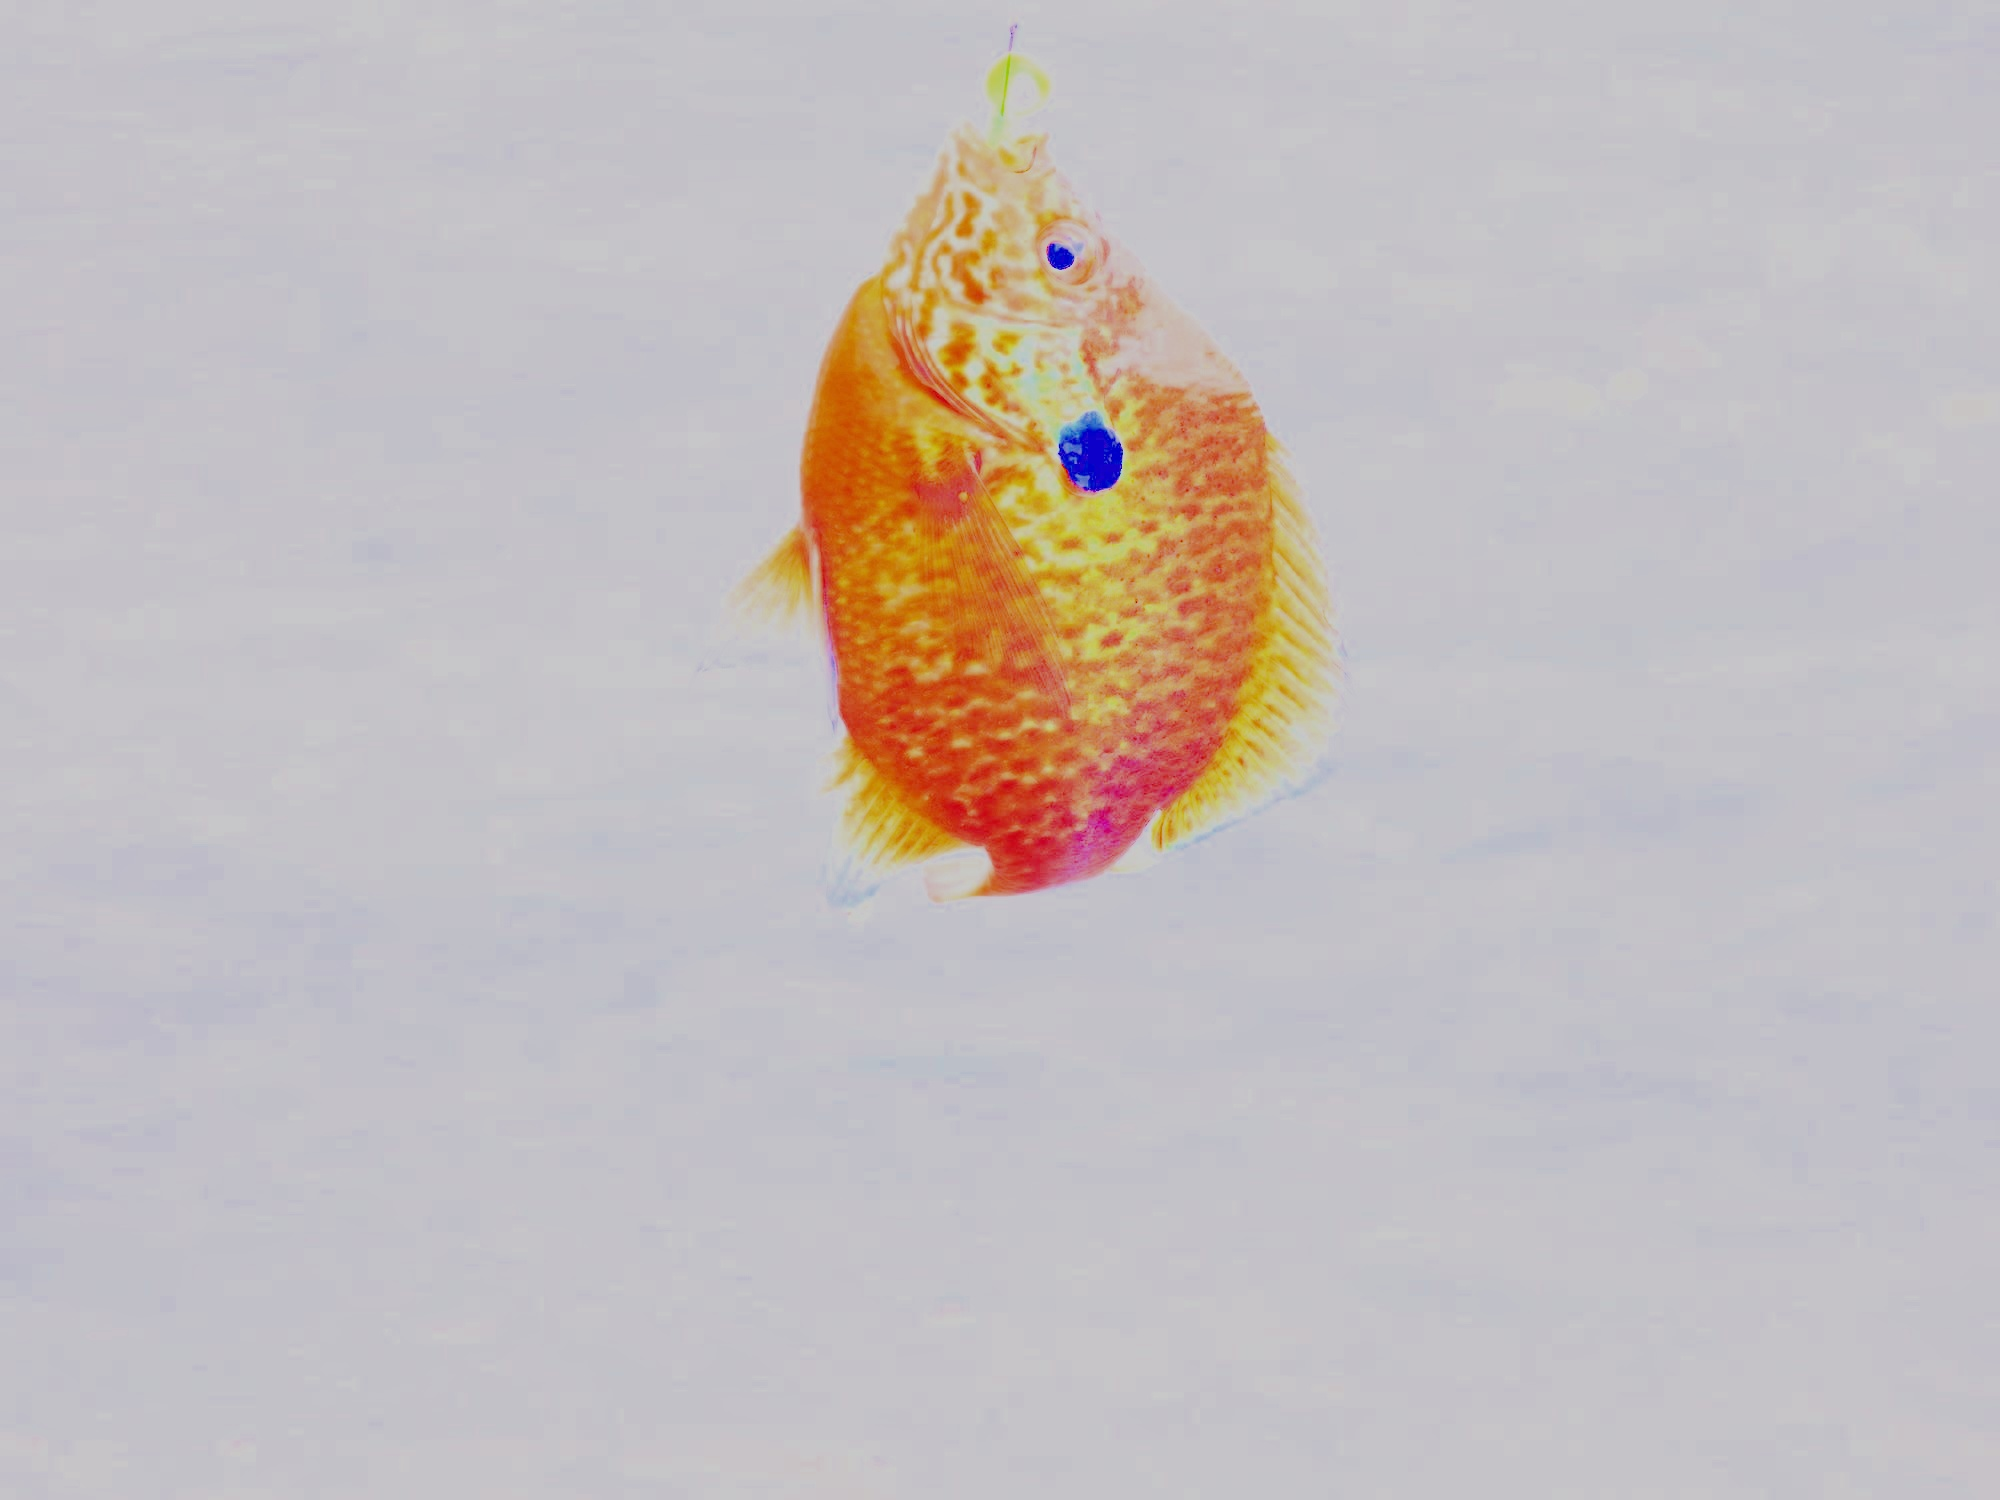
\includegraphics[width=.9\linewidth]{Images/shadow_removal}
        \caption{Shadow Removal}
    \end{subfigure}
    \caption{Example of shadow removal}
    \label{fig:shadow_removal}
\end{figure}

In figure \ref{fig:shadow_removal} it is shown that the colors of the fish is preserved, while all the shadows and blurry background in grey tones is evened out. In this example the value component is set to 200.

This type of simple shadow removal can be very useful, but for the image in figure \ref{fig:median_filter} the fish is not colorful enough for the technique to remove the shadows only.

